\documentclass[border=20pt,preview]{standalone}
\usepackage{tikz}
\usepackage{xcolor}

\definecolor{darkGray}{RGB}{192, 192, 192}
\definecolor{lightGray}{RGB}{229, 228, 226}

\begin{document}

\begin{center}
    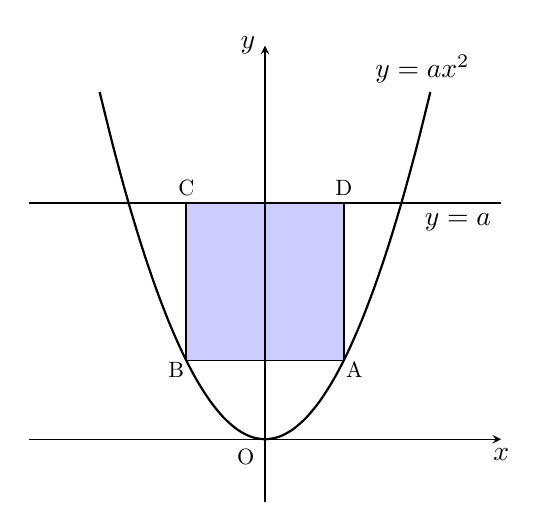
\begin{tikzpicture}
        \pgfmathsetmacro{\axislimit}{3}

        \fill[fill=blue!20] (1, 3) rectangle (-1, 1);

        \node[below left=1pt, scale=0.8] (origin) at (0,0) {\(\rm{O}\)};
        \draw [-stealth] (-\axislimit, 0) -- (\axislimit, 0) node[below] {\(x\)};
        \draw [-stealth] (0, -0.8) -- (0, 5) node[left] {\(y\)};

        \draw [thick] (-\axislimit, 3) -- (\axislimit, 3) node [below left] {\(y = a\)};

        \draw[thick, domain=-2.1:2.1, smooth, variable=\x] plot ({\x}, {\x * \x});

        \draw [semithick] (1, 3) rectangle (-1, 1);
        \node [below right=-2pt, scale=0.8] at (1, 1) {\(\rm{A}\)};
        \node [below left=-2pt, scale=0.8] at (-1, 1) {\(\rm{B}\)};
        \node [above, scale=0.8] at (-1, 3) {\(\rm{C}\)};
        \node [above, scale=0.8] at (1, 3) {\(\rm{D}\)};

        \node at (2, 4.7) {\(y = ax^2\)};
    \end{tikzpicture}
\end{center}

\end{document}
